\chapter{}
\section{Búsqueda en Scopus}
Se utiliza la siguiente combinación de búsqueda por terminología, palabras claves y conceptos relacionados con metrología de vista única: \begin{lstlisting}[language=,basicstyle=\ttfamily\small,breaklines=true,frame=single,backgroundcolor=\color{gray!10}]
(TITLE-ABS-KEY("single view metrology" OR "single-view metrology" OR "single image 3D reconstruction" OR "monocular 3D reconstruction" OR "geometry from a single image" OR "single view geometry"))
AND (LIMIT-TO(SUBJAREA, "COMP") OR LIMIT-TO(SUBJAREA, "ENG"))
AND (LIMIT-TO(DOCTYPE, "ar") OR LIMIT-TO(DOCTYPE, "cp"))
\end{lstlisting}

\section{Configuración por Localización}\label{app:LocationConfig}
\begin{table}[!ht]
\scriptsize
\centering
\begin{tabular}{|l|c|c|c|}
\hline
\rowcolor[HTML]{FFCB2F}
\textbf{Cámara} & \textbf{Altura (m)} & \textbf{Posición relativa a RS} \\
\hline
RS (RealSense) & 1.593 & (0, 0, 0) \\
\hline
Cam1 (Tapo C120) & 1.509 & (-0.4000, -0.0840, +0.4000) \\
\hline
Cam2 (Dahua) & -- & -- \\
\hline
Cam3 (Hikvision) & -- & -- \\
\hline
\end{tabular}
\caption{Posición de las cámaras en la sala de seminarios.}\label{tab:SeminarRoom}
\end{table}

\begin{table}[!ht]
\centering
\scriptsize
\begin{tabular}{|l|c|c|c|}
\hline
\rowcolor[HTML]{FFCB2F}
\textbf{Cámara} & \textbf{Altura (m)} & \textbf{Posición relativa a RS} \\
\hline
RS (RealSense) & 1.555 & (0, 0, 0) \\
\hline
Cam1 (Tapo C120) & 1.332 & (+0.4510, -0.2230, +1.9280) \\
\hline
Cam2 (Dahua) & 1.498 & (-0.7630, -0.0570, +1.4980) \\
\hline
Cam3 (Hikvision) & -- & -- \\
\hline
\end{tabular}
\caption{Posición de las cámaras en el aparcamiento.}\label{tab:ParkingLot}
\end{table}

\begin{table}[!ht]
\centering
\scriptsize
\begin{tabular}{|l|c|c|c|}
\hline
\rowcolor[HTML]{FFCB2F}
\textbf{Cámara} & \textbf{Altura (m)} & \textbf{Posición relativa a RS} \\
\hline
RS (RealSense) & 1.530 & (0, 0, 0) \\
\hline
Cam1 (Tapo C120) & 1.350 & (-0.6260, -0.1800, +0.2640) \\
\hline
Cam2 (Dahua) & 1.790 & (-0.4250, +0.2600, -0.1200) \\
\hline
Cam3 (Hikvision) & 2.250 & (-0.7100, +0.7200, -0.5950) \\
\hline
\end{tabular}
\caption{Posición de las cámaras en la acera.}\label{tab:Sidewalk}
\end{table}

\begin{table}[H]
\centering
\scriptsize
\begin{tabular}{|l|c|c|c|}
\hline
\rowcolor[HTML]{FFCB2F}
\textbf{Cámara} & \textbf{Altura (m)} & \textbf{Posición relativa a RS} \\
\hline
RS (RealSense) & 1.810 & (0, 0, 0) \\
\hline
Cam1 (Tapo C120) & -- & -- \\
\hline
Cam2 (Dahua) & -- & -- \\
\hline
Cam3 (Hikvision) [idai10] & 2.050 & (-1.2130, +0.2400, 0) \\
\hline
Cam3 (Hikvision) & 2.050 & (-1.2130, +0.2400, +0.6120) \\
\hline
\end{tabular}
\caption[Posición de las cámaras en la rampa de entrada.]{Posición de las cámaras en la rampa de entrada. Hay un posicionamiento distinto para la cámara 3, para 1 sujeto específico (idai10).}\label{tab:EntranceRamp}
\end{table}

\section{Utilizando Detectron2}\label{app:YAMLConfig}
El sistema de configuración de \emph{Detectron2}~\cite{detectron2} se basa en una arquitectura jerárquica de ficheros YAML.
En dichos ficheros, se definen parámetros de entrenamiento, arquitectura, conjuntos de datos, optimización y evaluación de forma centralizada.
De esta forma, es posible llevar a cabo un seguimiento del historial de cambios en experimentos a través de herramientas como Git, así como
la creación de variantes sin redundancia al utilizar el sistema de herencia, simplificando el mantenimiento y la comparación sistemática de experimentos.
En el Ejemplo~\ref{lst:ROIHYaml}, se observa la configuración de la experimentación del modelo de estimación de la altura.
\par
Otro mecanismo principal que habilita una flexibilidad experimental recae sobre el sistema de registros, entre los que
destacan \lstinline{META_ARCH_REGISTRY}, encargado de asociar identificadores a arquitectura de modelos, el registro \lstinline{ROI_HEADS_REGISTRY},
que agrupa los identificadores de los módulos de estimación sobre las regiones de interés,
y, por último, \lstinline{BACKBONE_REGISTRY}, que permite configurar diferentes esqueletos de extracción de características principales.
Gracias a este patrón, un nuevo modelo puede integrarse simplemente registrando una clase derivada de la arquitectura base y
realizando únicamente las modificaciones pertinentes.
Además, cada componente puede extenderse de forma independiente y posteriormente ensamblarse sin necesidad de
modificar el flujo general de entrenamiento (véase el Ejemplo~\ref{lst:ModelRegistry}).
Como consecuencia, una vez registradas las nuevas clases y actualizada la configuración, el modelo puede entrenarse
directamente utilizando los procedimientos de entrenamiento ya definidos. A su vez, se puede extender
la clase encargada de realizar el entrenamiento para incluir procedimientos adicionales (como es el caso
del entrenamiento en precisión mixta).

\noindent\begin{minipage}{\textwidth}
\begin{lstlisting}[
language=Python,
basicstyle=\scriptsize,
captionpos=b,
caption={
[Ejemplo de extensión de módulos de estimación en Detectron2~\cite{detectron2}.]
Ejemplo de extensión de módulos de estimación en Detectron2~\cite{detectron2}.
Una vez registrado el nuevo módulo de estimación de camera en \lstinline{ROI_HEADS_REGISTRY}
(que extiende el comportamiento habitual de \lstinline{ROI_HEADS}), modificamos el archivo de
configuración del experimento para hacer uso de la misma y poder lanzar el entrenamiento,
sin tener que modificar nada más.
},
  label={lst:ModelRegistry},
]
@ROI_HEADS_REGISTRY.register()
class CameraHead(ROIHeads):
  """Clase que herada de ROIHeads, extendiendo el metodo forward"""
    def forward(
      self,
      features: Dict[str, torch.Tensor],
      proposals: List[Instances],
      targets: Optional[List[Instances]] = None,
  ) -> Tuple[List[Instances], Dict[str, torch.Tensor]]:
      features = [features[f] for f in self.box_in_features]
      box_features = self.box_pooler(features, [x.proposal_boxes for x in proposals])
      x = self.predictor(box_features)
      class_logits = self.cls_score(x)
      losses = {}
      if self.training:
        # My custom loss function
        losses = self.compute_loss(class_logits, targets)
      return class_logits, losses
\end{lstlisting}
\end{minipage}


\section{Visualización del entrenamiento}\label{app:VisualizeTraining}
Otra demostración de la extensibilidad de la implementación en \emph{Detectron2}~\cite{detectron2} es
la posibilidad de redefinir o modificar flujos existentes por medio de la sobrecarga de
funciones y métodos, sin tener que modificar la lógica principal del código. Un ejemplo de ello
es la sobrecarga del método \lstinline{visualize_training} de la meta-arquitectura que permite
guardar visualizaciones de las estimaciones del modelo durante el entrenamiento. Esto permite
realizar un análisis cualitativo del proceso de aprendizaje del modelo.
En la Figura~\ref{fig:VisualizeTraining},
se observan cómo las predicciones del módulo de estimación de parámetros de la cámara son cada vez más precisas durante el entrenamiento.
\par
Esto es posible debido al uso de Tensorboard~\cite{Tensorflow}, una herramienta de monitorización ampliamente
utilizada en aprendizaje profundo. Tensorboard permite registrar y visualizar de forma interactiva distintos
tipos de información generada durante el entrenamiento, incluyendo imágenes, métricas, histogramas y grafos
computacionales. Combinando tanto métricas cuantitativas como cualitativas en una única interfaz.
Esto facilita la detección temprana de problemas, comparación entre experimentos y eficiencia del proceso
de desarrollo de modelos de aprendizaje profundo.
\section{Lanzar experimentos}\label{app:LaunchExperiments}
Una vez creada las diferentes configuraciones de los experimentos, se puede lanzar el
entrenamiento utilizando un único script e indicando la configuración a utilizar (véase el Ejemplo~\ref{lst:LaunchTrain}). Para
este proyecto se han creado las siguientes configuraciones:
\begin{enumerate}
  \itemsep0cm
  \item \emph{calib.yaml}: configuración de entrenamiento sobre Pano360~\cite{SPEC}, para estimar los parámetros de la cámara.
  \item \emph{coco-scale.yaml}: configuración de entrenamiento sobre COCO-Scale~\cite{SVMIW}, para la detección y estimación de pose de humanos.
  \item \emph{coco-scale-calib.yaml}: configuración de entrenamiento híbrida sobre Pano360~\cite{SPEC} y COCO-Scale~\cite{SVMIW}, para estimación de parámetros de la cámara y detección de humanos.
  \item \emph{coco-scale-calib-roih.yaml}: configuración de entrenamiento híbrida final, sobre Pano360~\cite{SPEC} y COCO-Scale~\cite{SVMIW}, en la que se estima la altura de los humanos.
\end{enumerate}
Dichas ejecuciones se pueden concatenar haciendo uso del conector de ejecuciones exitosas de Linux (``\lstinline{&&}''). De
esta forma, obtener el modelo desarrollado desde cero, con todas sus fases, consistiría en concatenar la ejecución del
Ejemplo~\ref{lst:LaunchTrain}, utilizando solamente los argumentos ~\lstinline{--num-gpus} y~\lstinline{--config-file},
asignando las configuraciones en el orden correspondiente: calib.yaml, coco-scale-calib.yaml y coco-scale-calib-roih.yaml.
\begin{lstlisting}[
basicstyle=\scriptsize,
captionpos=b,
caption={
[Ejemplo de ejecución simples del código de entrenamiento.]
Ejemplo de ejecución simples del código de entrenamiento.
Se definen el número de tarjetas gráficas a utilizar (\lstinline{--num-gpus}),
el archivo de configuración de referencia (\lstinline{--config-file}) y algunas configuraciones manuales,
para sobre-escribir a las de dicho archivo.
En este ejemplo, se ejecutaría el entrenamiento del módulo de estimación de parámetros de la cámara.
Además, se sobre-escriben dónde guardar los resultados (\lstinline{OUTPUT-DIR}),
el ratio de aprendizaje (\lstinline{SOLVER.BASE_LR}) y el número de imágenes por iteración (\lstinline{SOLVER.IMS_PER_BATCH}).
},
  label={lst:LaunchTrain},
]
python train_calib.py --num-gpus 1 \
--config-file ./configs/COCO-Scale/calib.yaml \
OUTPUT_DIR output/calibrar-camera
SOLVER.BASE_LR 0.002343 SOLVER.IMS_PER_BATCH 12
\end{lstlisting}

\begin{figure}[!htp]
  \begin{center}
    \subfloat{\includegraphics[width=0.95\textwidth]{imagenes/appendix/visualize/visualize_2000.png}}\\
    \subfloat{\includegraphics[width=0.95\textwidth]{imagenes/appendix/visualize/visualize_10000.png}}\\
    \subfloat{\includegraphics[width=0.95\textwidth]{imagenes/appendix/visualize/visualize_18000.png}}\\
  \end{center}
  \caption[Visualización del entrenamiento de estimación de parámetros de cámara.]{
  Visualización del entrenamiento de estimación de parámetros de cámara.
  Cada par de imágenes representa el valor real (a la izquierda) y el valor estimado (a la derecha).
  Se observa desde el principio del entrenamiento (primera fila), hasta finales del mismo (última fila).
  Este tipo de registro continuo durante el entrenamiento nos permite hacer un análisis cualitativo
  del comportamiento del modelo durante el entrenamiento. La combinación de este análisis con el cuantitativo,
  de observar las funciones de pérdida y métricas de evaluación, nos permite tomar mejores decisiones.
}\label{fig:VisualizeTraining}
\end{figure}


\noindent\begin{minipage}{\textwidth}
\begin{lstlisting}[
  style=YAML,
  captionpos=b,
  caption={
  [Ejemplo de configuración del método de estimación de la altura.]
  Ejemplo de configuración del método de estimación de la altura.
  Se observa el sistema jerárquico de \emph{Detectron2}~\cite{detectron2},
  dado que partimos del archivo raíz (\lstinline{__BASE__}) de su modelo de
  detección de poses. Se ha configurado una meta-arquitectura (\lstinline{META_ARCHITECTURE})
  personalizada en la que se emplea los módulos de estimación sobre regiones de interés
  propuestas (\lstinline{ROI_HEADS}) que incluyen la estimación de la altura de los objetos
  (\lstinline{HeightStandardROIHeads}). Los pesos de las pérdidas son fácilmente
  ajustables (cadenas que incluyen la palabra \lstinline{LOSS}), así como elegir
  realizar, o no, el entrenamiento en precisión mixta (\lstinline{AMP}).
  },
  label={lst:ROIHYaml},
]
_BASE_: "../COCO-Keypoints/keypoint_rcnn_R_50_FPN_3x.yaml"
MODEL:
  WEIGHTS: "output/kpsbbox-calib-v2/model_final.pth"
  META_ARCHITECTURE: "GeneralizedCamRCNN"
  ROI_HEADS:
    NAME: "HeightStandardROIHeads"
  ROI_BOX_HEAD:
    BBOX_REG_LOSS_WEIGHT: 10.0
  ROI_KEYPOINT_HEAD:
    NAME: "KRCNNConvDeconvUpsampleHead"
    LOSS_WEIGHT: 10.0
  KEYPOINT_ON: False
  HEIGHT_ON: True
  POINT_NET_ON: True
  HEIGHT_REFINE_ON: True
  HEIGHT_HEAD:
    LOSS_WEIGHT: 0.05
    SMOOTH_L1_BETA: 0.1
  POINT_NET:
    POOLING: "max"
    TEMPERATURE: 1.0
    BN: False
    TRANSFORM: True
    DETACH: False
    REFINE_TEMPERATURE: 1.0
    REFINE_LAYERS: 2
DATASETS:
  TRAIN: ("COCOScale2017Calib_train", )
  TEST: ("COCOScale2017_val", "Pano360_val", )
SOLVER:
  IMS_PER_BATCH: 6
  RATIO_PANO360: (3, 1)  # 3 COCO, 1 CALIB
  BASE_LR: 0.007031
  STEPS: (60000, 80000)
  MAX_ITER: 90000
  AMP:
    ENABLED: True
  CLIP_GRADIENTS:
    CLIP_TYPE: norm
    CLIP_VALUE: 1.0
    ENABLED: true
    NORM_TYPE: 2.0
TEST:
  EVAL_PERIOD: 2000
DATALOADER:
  NUM_WORKERS: 2
  FILTER_EMPTY_ANNOTATIONS: False
  ASPECT_RATIO_GROUPING: True
VIS_PERIOD: 500
FLOAT32_PRECISION: "medium"
SEED: 140421
\end{lstlisting}
\end{minipage}

\section{Generación de datos}\label{app:DataDistribution}
En~\cite{SVMIW, CalibDataGeneration} muestrean los valores de manera controlada, incluyendo
la distancia focal y la orientación de la cámara (ángulo de alabeo, de elevación y guiñada).
En lugar de utilizar una distribución uniforme para todos los parámetros, el muestreo se diseña
con objetivo de cubrir de forma equilibrada el espacio de configuraciones perceptualmente relevantes,
evitando la sobre representación de determinados rangos.
Destaca la distribución de alabeo que utiliza dos distribuciones de Cauchy con valores
muy centrados en cero (véase la Figura~\ref{fig:AngleDistSVMIW}),
con fin de modelar el hecho de que la mayoría de las fotos tienen ese ángulo a cero.
De forma similar, la relación de aspecto es extraída de imágenes presentes en Flickr e ImageNet~\cite{ImageNet}, asignando
mayor probabilidad a los tipos más comunes (por ejemplo, un 66\% al ratio 4:3).

\begin{figure}[!htp]
  \begin{center}
    \subfloat{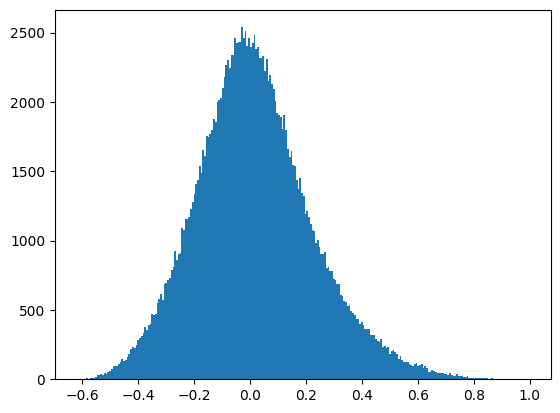
\includegraphics[width=0.45\textwidth]{imagenes/appendix/pitch_scale_dist.png}}
    \subfloat{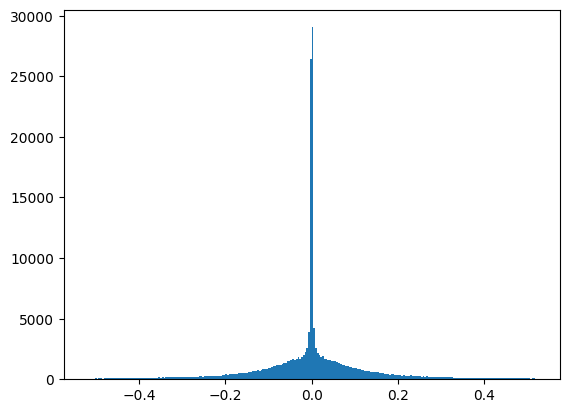
\includegraphics[width=0.45\textwidth]{imagenes/appendix/roll_scale_dist.png}}\\
    \subfloat{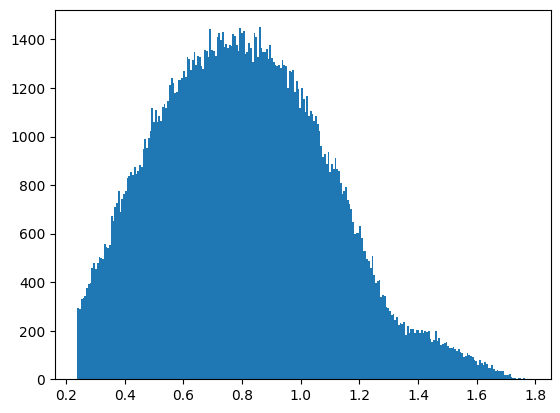
\includegraphics[width=0.45\textwidth]{imagenes/appendix/vfov_scale_dist.png}}
  \end{center}
  \caption[Visualización de distribución de ángulos de cámara utilizado por~\cite{SVMIW}, basado en~\cite{CalibDataGeneration}.]{
  Visualización de distribución de ángulos de cámara utilizado por~\cite{SVMIW}, basado en~\cite{CalibDataGeneration}.
  Primeramente, tenemos al ángulo de elevación, seguido del de alabeo y, por último, el valor del campo de visión vertical.
  Se generan 7 ejemplos por cada panorámica, para un total de 187.206 imágenes de entrenamiento y 5000 para validación.
  Destaca el ángulo de alabeo (imagen superior derecha) que sigue una distribución de Cauchy muy centrada en cero, pudiendo
  ocasionar que el modelo no aprenda a estimar adecuadamente valores diferentes.
}
  \label{fig:AngleDistSVMIW}
\end{figure}

En~\cite{SPEC} se inspiran en el método anterior, pero asignan distribuciones
normales a cada parámetro de la cámara (véase la Figura~\ref{fig:AngleDistSPEC}).
Esta elección es la utilizada en este proyecto para poder hacer la comparativa de los resultados
ilustrados por el mismo artículo~\cite{SPEC}, en el cual se incluye también resultados estimados por
los autores de~\cite{SVMIW} (método desarrollado en este documento).
Además, en~\cite{CNNFragility} observaron que utilizar datos equilibrados mejoran la capacidad de generalización
de redes convolucionales, permitiendo el modelo aprender a extraer características que realmente codifican la
información necesaria para estimar correctamente las clases minoritarias. Cuanto mayor es el desequilibrio
entre las clases (o de los valores a estimar), más suele el modelo recurrir a memorizar los ejemplos que
rara vez ocurren en lugar de aprender a interpretarlos. Por lo tanto, utilizar este método nos permite
facilitar la tarea de aprendizaje del modelo, su capacidad de generalización y comparar nuestra implementación con
algunos resultados de referencia.

\begin{figure}[!htp]
  \begin{center}
    \subfloat{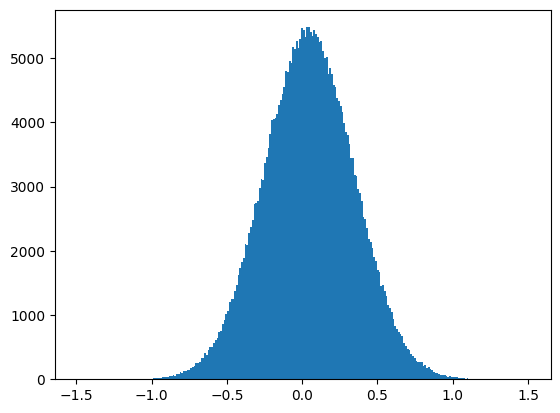
\includegraphics[width=0.45\textwidth]{imagenes/appendix/pitch_spec_dist.png}}
    \subfloat{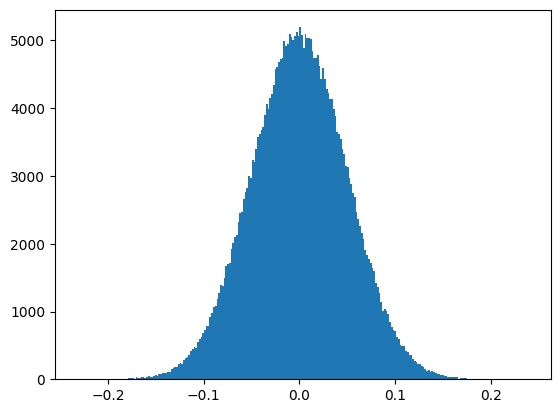
\includegraphics[width=0.45\textwidth]{imagenes/appendix/roll_spec_dist.png}}\\
    \subfloat{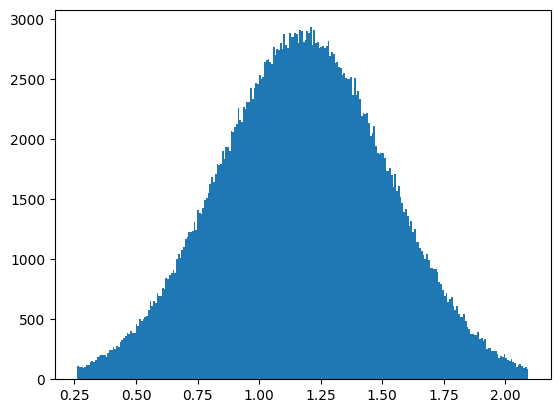
\includegraphics[width=0.45\textwidth]{imagenes/appendix/vfov_spec_dist.png}}
  \end{center}
  \caption[Visualización de distribución de ángulos de cámara utilizado por~\cite{SPEC}.]{
  Visualización de distribución de ángulos de cámara utilizado por~\cite{SPEC}.
  Primeramente, tenemos al ángulo de elevación, seguido del de alabeo y, por último, el valor del campo de visión vertical.
  Se generan 12 ejemplos por cada panorámica, para un total de 347.304 imágenes de entrenamiento y 12.732 de validación.
  A diferencia del método de generación empleado por~\cite{SVMIW}, basado en~\cite{CalibDataGeneration},
  todos los ángulos siguen una normal, facilitando la tarea de aprendizaje del modelo de estimación
  de parámetros de la cámara.
}
  \label{fig:AngleDistSPEC}
\end{figure}
